% !TeX root = ../dokumentation.tex

\chapter{Projekt Ergebnisse}

\section{Erreichte Ziele}

\section{Analyse der Organisatorischen Änderungen}

\subsection{Kapazitätsschätzungen}

Zu Beginn des Projektes gab es Schwierigkeiten mit der Planung des Sprintumfangs.
Im ersten Sprint konnten vorgenommene Tickets nicht abgeschlossen werden. 
Dadurch konnte das Sprintziel nicht erreicht werden (vgl. Abbildung~\ref{fig:SKIOS-Sprint-1-Brundown}).

\begin{figure}[h]
    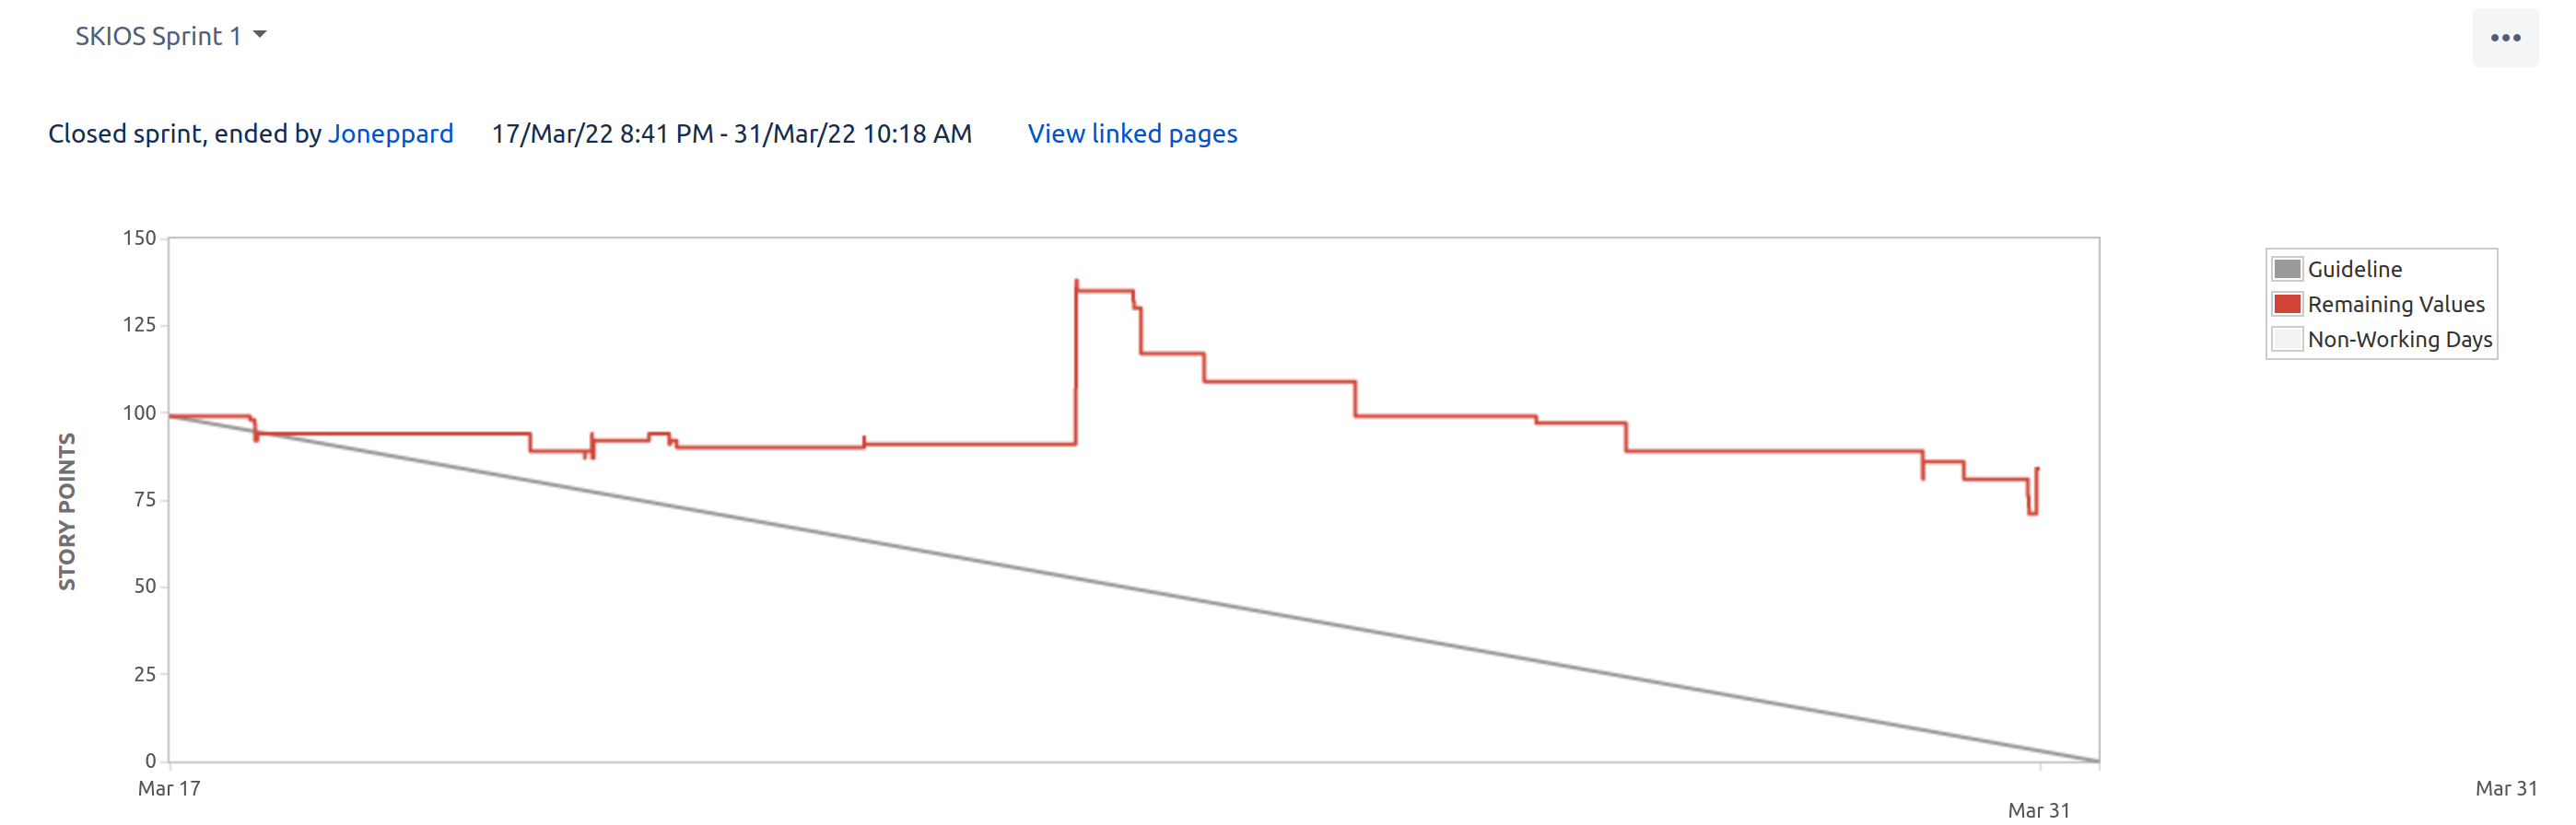
\includegraphics[width=\linewidth]{SKIOS-Sprint-1-Brundown-Diagram.png}
    \caption{Brundown-Chart zu Sprint 1}
    \label{fig:SKIOS-Sprint-1-Brundown}
\end{figure}

Unter anderem wurde in der Retrospektive daraufhin festgehalten, 
dass sich die Kapazitäten zwischen den einzelnen Teammitgliedern sehr stark unterschieden.
Für den Sprint 1 ist man davon ausgegangen, dass jedes Teammitglied 20 Storypoints im Sprint bearbeiten kann.
Damit genauer geplant werden kann, wurde im Confluence eine Seite zur Kapazitätsschätzung eingerichtet.
Dabei handelt es sich um eine Tabelle, in der jedes Teammitglied in Storypoints die eigene Kapazität einschätzen konnte.
Diese wurde wie in Abbildung~\ref{fig:Capacitytable} erstellt. 

\begin{figure}[h]
    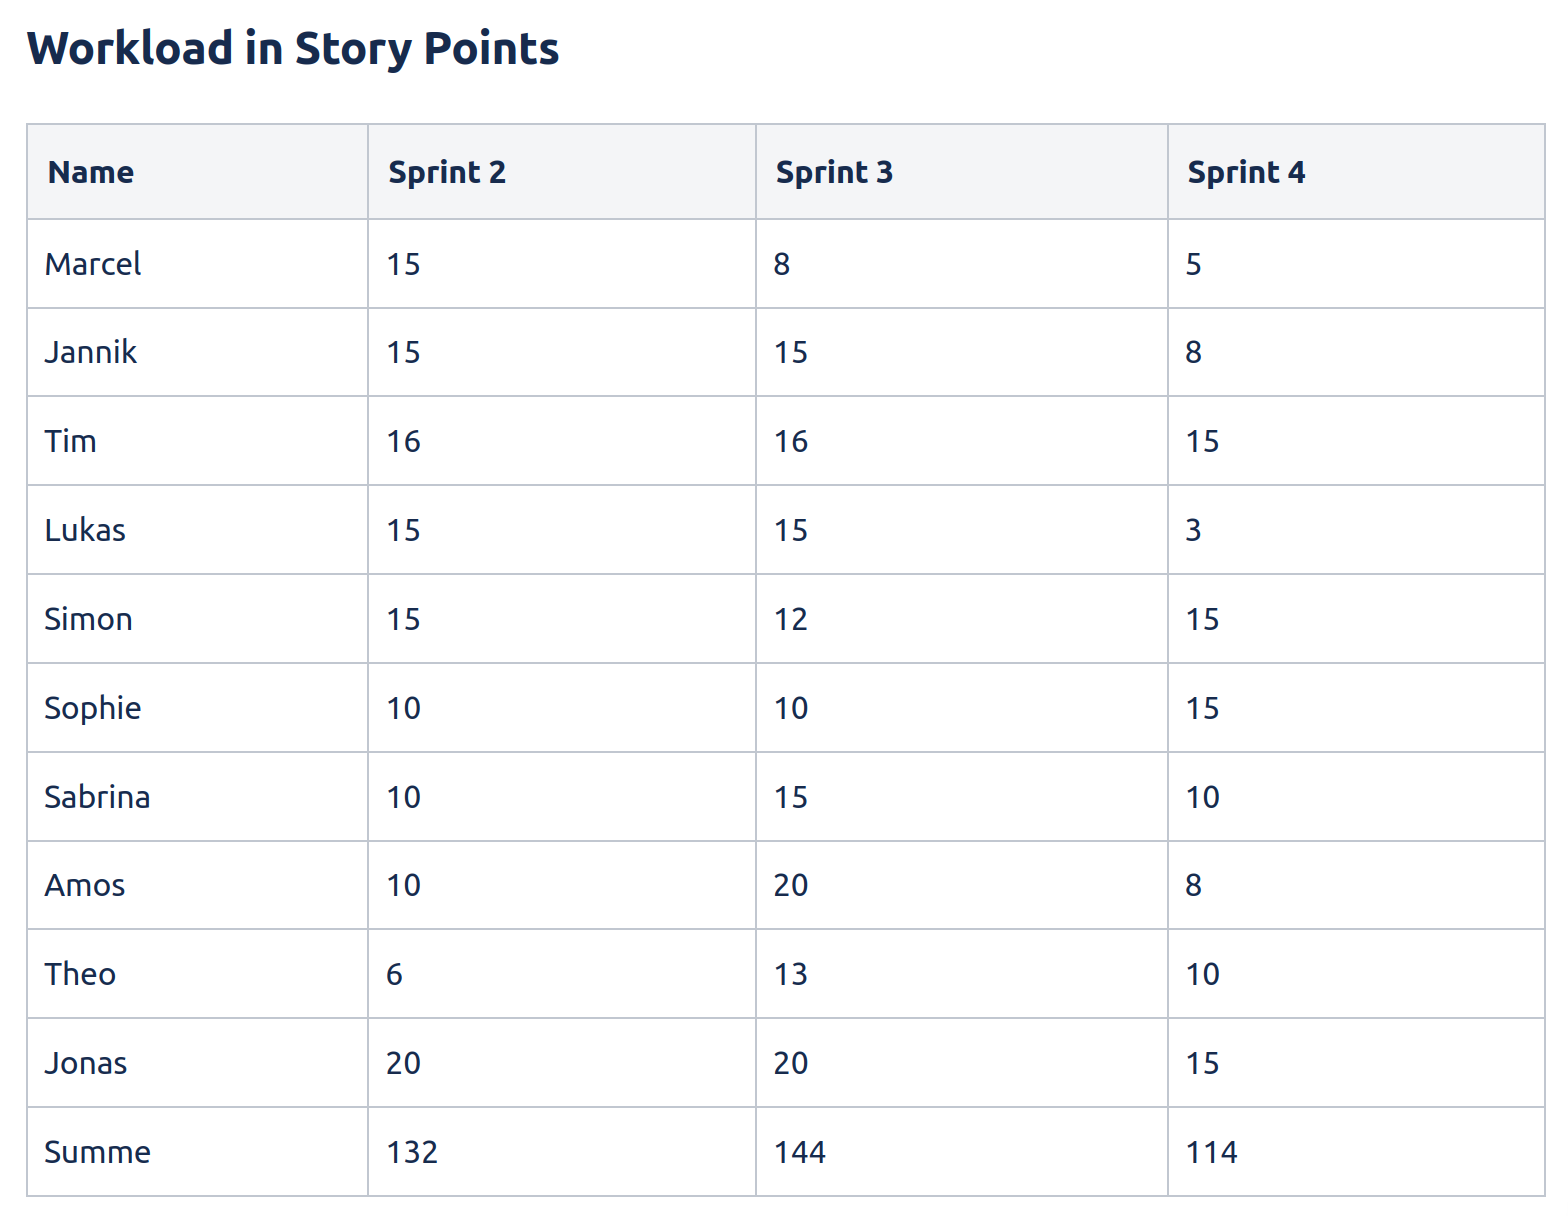
\includegraphics[width=\linewidth]{SKIOS-Capacity-Esitmates.png}
    \caption{Kapazitätschätzungen der Teammitglieder}
    \label{fig:Capacitytable}
\end{figure}

Mit einer besseren Kapazitätsschätzung konnten im nächsten Sprint, dann auch deutlich mehr vorgenommene Tickets abgeschlossen werden (vgl. Abbildung~\ref{fig:SKIOS-Sprint-2-Burndown}).
Es war möglich zumindest vorhersehbare Ereignisse, die die Kapazität einzelner stark einschränken, abzufangen.
Im dritten Sprint wurden auch die Schätzungen der eigenen Kapazität besser, wodurch dann auch das Sprintziel erreicht wurde (vgl. Abbildung~\ref{fig:SKIOS-Sprint-3-Burndown}).

\begin{figure}[H]
    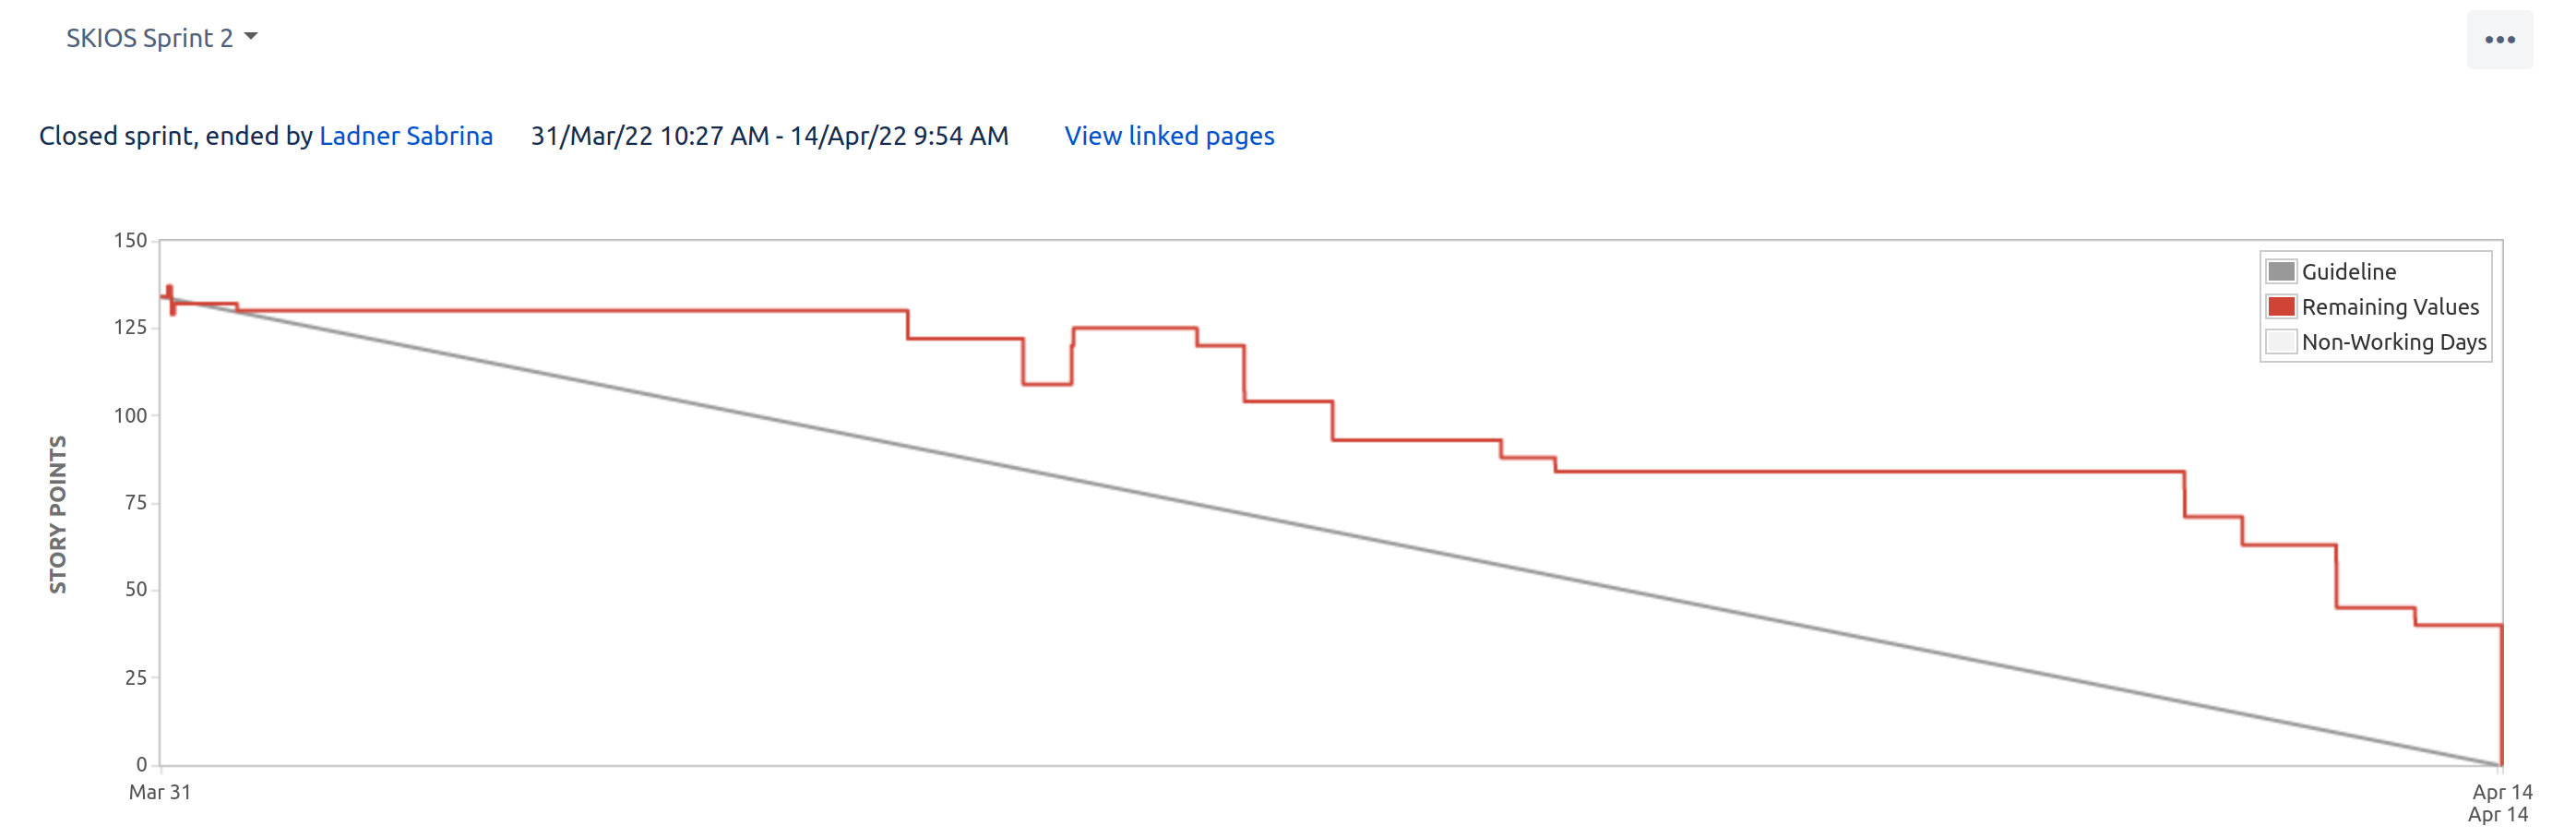
\includegraphics[width=\linewidth]{SKIOS-Sprint-2-Brundown-Diagram.png}
    \caption{Burndown-Chart zu Sprint 2}
    \label{fig:SKIOS-Sprint-2-Burndown}
\end{figure}

\begin{figure}
    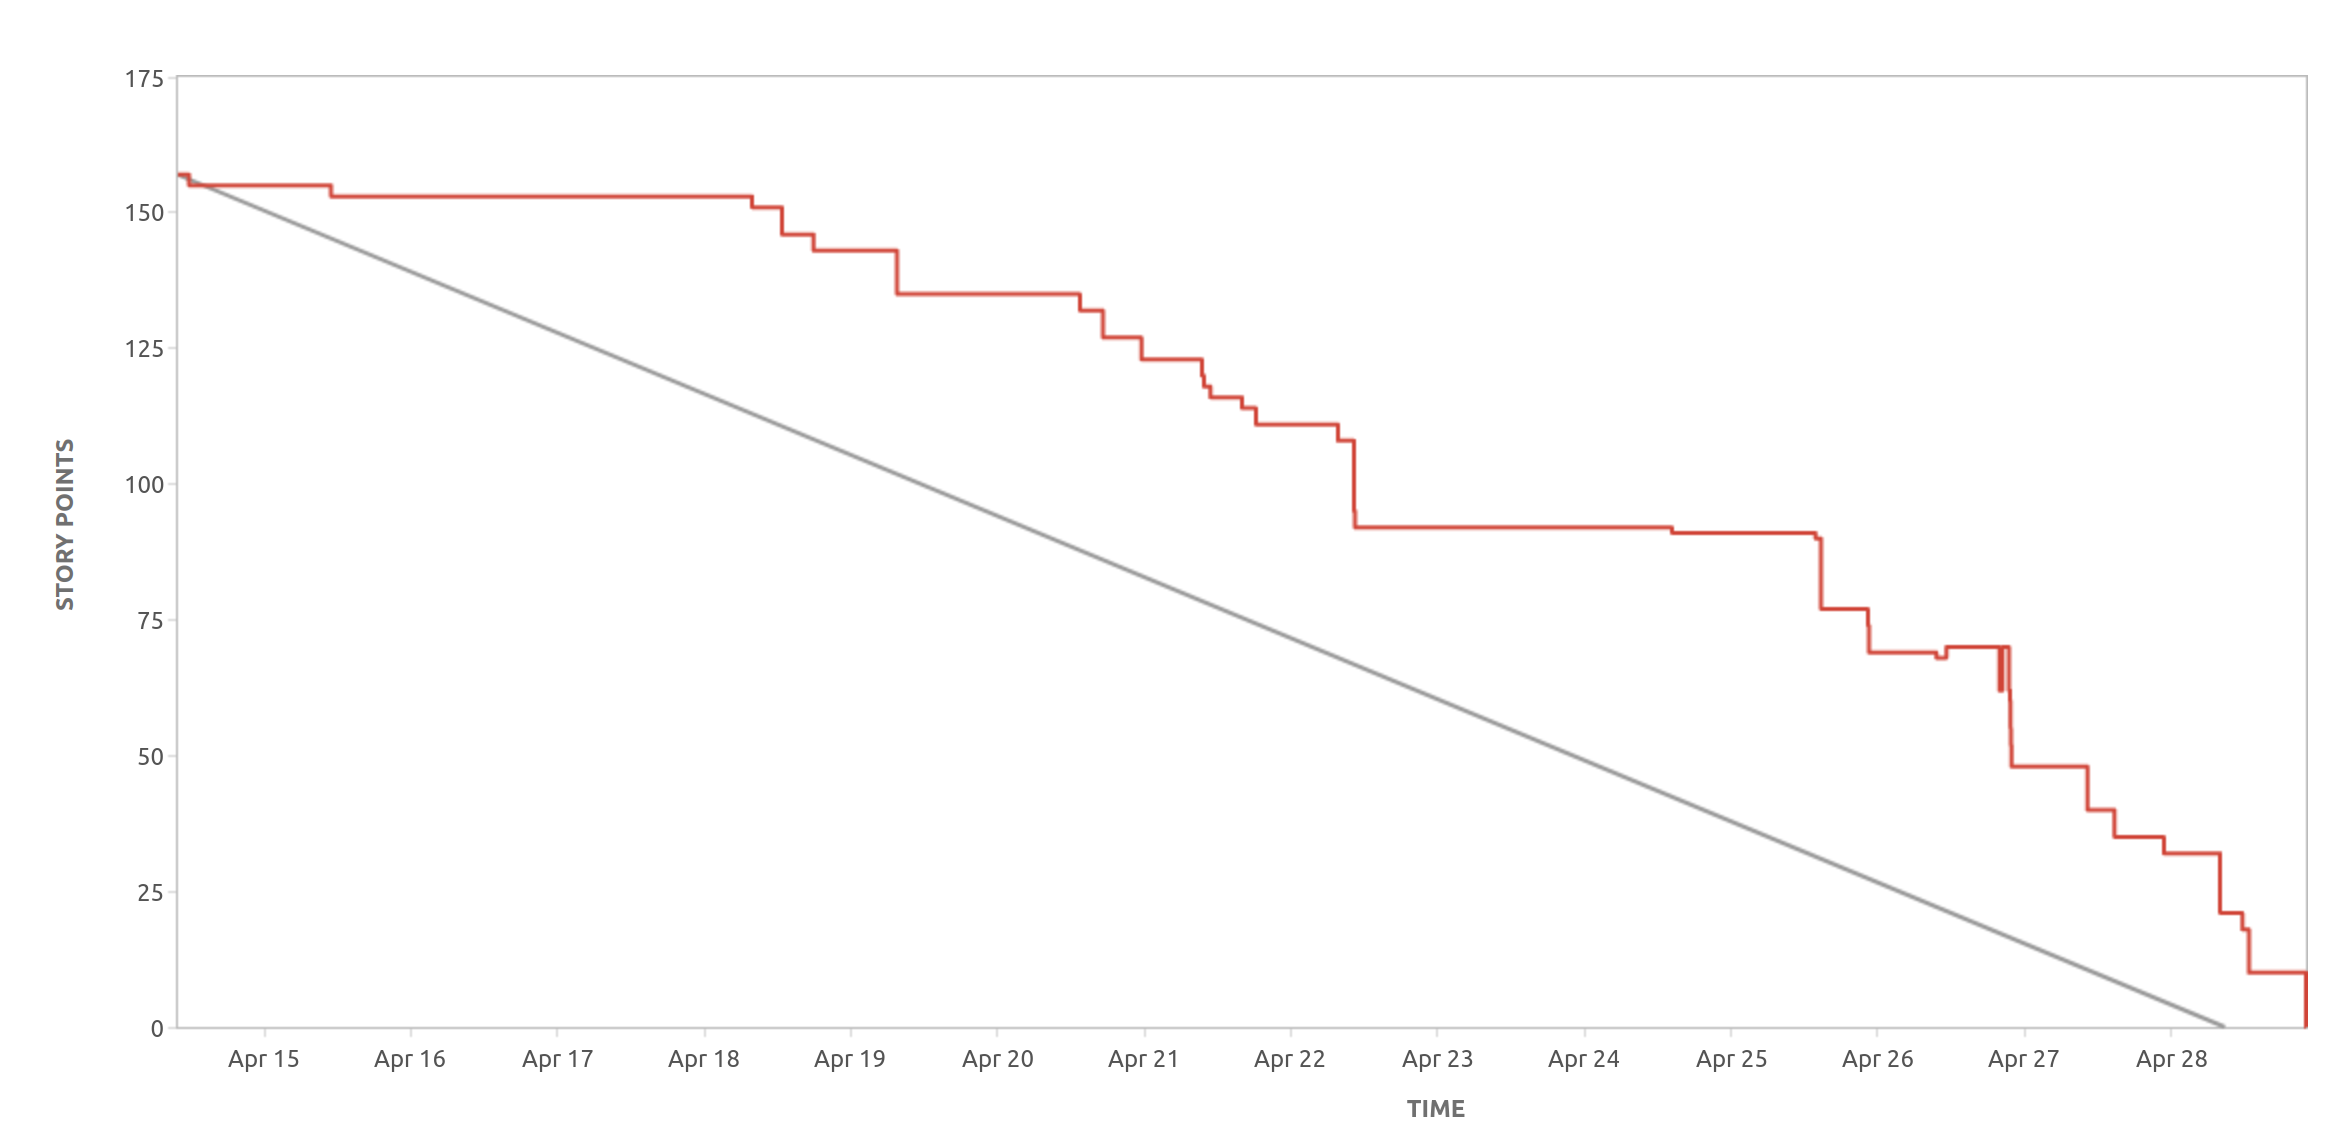
\includegraphics[width=\linewidth]{Skios-Sprint-3-Burndown-Chart.png}
    \caption{Burndown-Chart zu Sprint 3}
    \label{fig:SKIOS-Sprint-3-Burndown}
\end{figure}

\subsection{WIP-Limits}
Zu Anfang des Projektes wurden sehr hohe Initialwerte für die \ac{WIP}-Limits gesetzt.
Das Problem hiermit verdeutlicht sich am besten an der \enquote{Needs Review} Swimlane.
Wie sich in Abbildung \ref{fig:WIP} (dem \ac{WIP}-Chart des Projektes) zeigt, hingen zum Anfang des ersten Sprints ein Großteil der Stories in diesem Status.

\begin{figure}
    \centering
    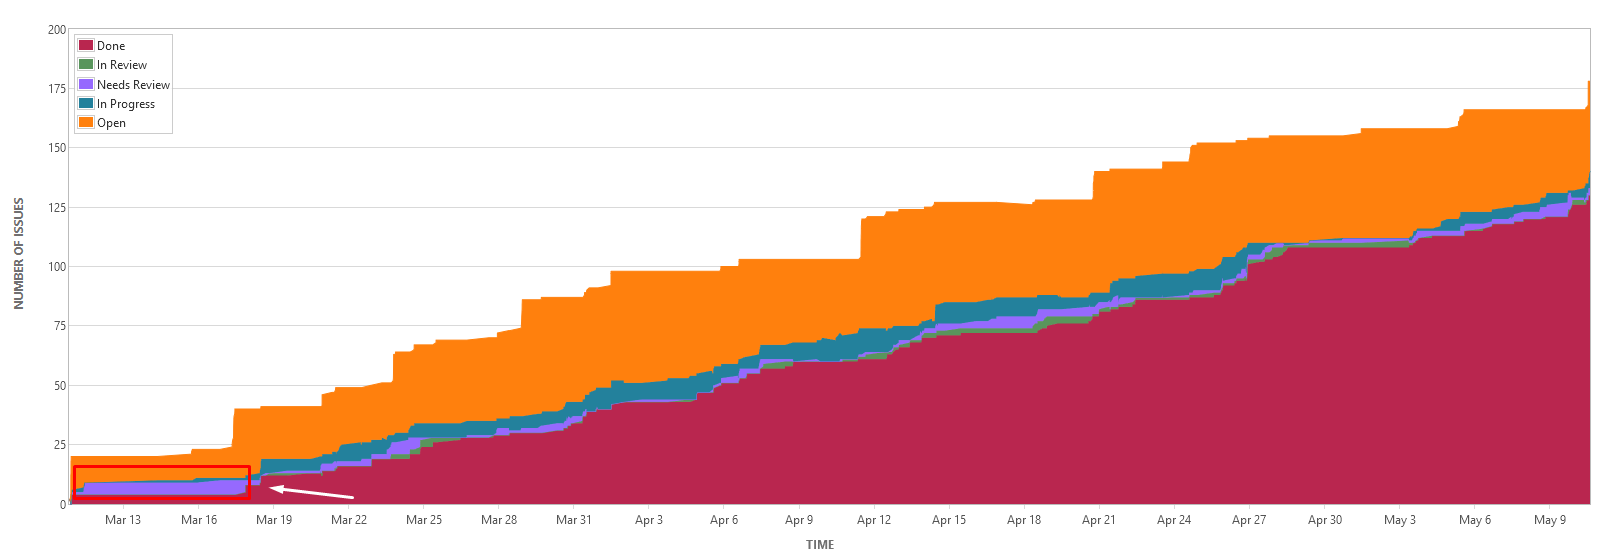
\includegraphics[width=\linewidth]{WIP-Chart.png}
    \caption{WIP Chart des Projektes}
    \label{fig:WIP}
\end{figure}

Als jedoch das \ac{WIP}-Limit dieser Swimlane von 11 auf 4 verringert wurde, ist die Aufhäufung an Tickets dem Team deutlicher geworden.
Im \ac{WIP}-Chart ist ebenfalls eindeutig zu erkennen, dass die Häufung (im Rot umrandeten Bereich) am Anfang sehr prävalent war, sich aber schlagartig zum Zeitpunkt des Einsetzten des Limits zurückgebildet hat (siehe weißer Pfeil).

\todo{Änderungen des Ablaufes erläutern und analysieren}

\subsection{Ausgliederung der Estimations aus den Planungsbesprechungen}

Innerhalb des Ersten Sprintes haben wir sehr viel Zeit für die Kapazitätschätzung benötigt. 
Dies hatte zur Folge, dass im Sprint Planning kaum Zeit für produktive Diskussionen übrig war und mit laufender Dauer die Konzentration für Estimations abnahm.
Daher haben wir beschlossen das Estimation Meeting vom Sprint Planning zu entkoppeln.
So kamen zu den den Bi-Weeklys und ungenutzten Vorlesungsterminen das neue Estimation Meeting hinzu.
Dies führte dazu, dass im Planning Meeting nun genügend Zeit war und die Qualität der Estimations zunahm, was sich in den Burndown-Charts reflektiert.

\section{Personenbeiträge}
(Zusammenfassung genau beschrieben in den jeweiligen Tickets der Sprints)